
\documentclass{beamer}
\usetheme{Madrid}
\usepackage{fontspec}
\usepackage{xunicode}
\usepackage{xltxtra}
\usepackage{xecyr}
\usepackage{hyperref}
\setmainfont[Mapping=tex-text]{DejaVu Serif}
\setsansfont[Mapping=tex-text]{DejaVu Sans}
\setmonofont[Mapping=tex-text]{DejaVu Sans Mono}
\usepackage{polyglossia}
\setdefaultlanguage{russian}
\usepackage{graphicx}
\usepackage{listings}
\lstdefinestyle{mycode}{
  belowcaptionskip=1\baselineskip,
  breaklines=true,
  xleftmargin=\parindent,
  showstringspaces=false,
  basicstyle=\footnotesize\ttfamily,
  keywordstyle=\bfseries,
  commentstyle=\itshape\color{gray!40!black},
  stringstyle=\color{red},
  numbers=left,
  numbersep=5pt,
  numberstyle=\tiny\color{gray},
}
\lstset{escapechar=@,style=mycode}

\begin{document}

\title[Бакалаврская работа]{Рандомизированный алгоритм при обработке данных ультразвуковых исследований}

\author[Иван Сенин]{
    \begin{flushright}
    Иван Сенин \\
    {\footnotesize\textcolor{gray}\raggedleft{группа 444\\Научный руководитель:\\д.\,ф.-м.\,н., профессор О.\,Н. Граничин}}
    \end{flushright}
}

\institute{СПбГУ}
\date{}


\frame{\titlepage}

\begin{frame}
\frametitle{Введение}
\framesubtitle{Ультразвуковая томография}


\begin{figure}[!ht]
\begin{flushleft}
  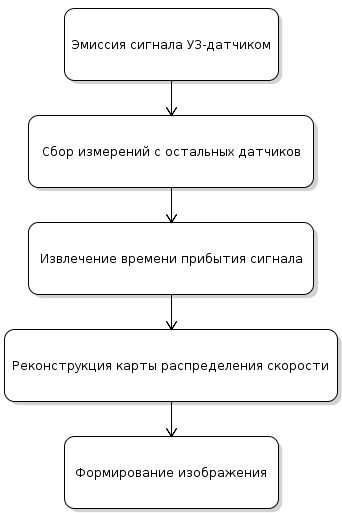
\includegraphics[scale=0.4]{pics/us_process.png}
\end{flushleft}
\end{figure}




\end{frame}


\begin{frame}\frametitle{Алгоритм}



\end{frame}

\begin{frame}\frametitle{Результаты}
\Large
\begin{itemize}
    \item Достигли
    \begin{itemize}
        \item того
        \item сего
    \end{itemize}
    \item Получили
    \item Обнаружили
\end{itemize}
\end{frame}



\begin{frame}
\end{frame}

\end{document}